% Created 2018-01-18 Thu 13:11
\documentclass[a4paper]{article}
\usepackage[utf8]{inputenc}
\usepackage[T1]{fontenc}
\usepackage{fixltx2e}
\usepackage{graphicx}
\usepackage{longtable}
\usepackage{float}
\usepackage{wrapfig}
\usepackage{rotating}
\usepackage[normalem]{ulem}
\usepackage{amsmath}
\usepackage{textcomp}
\usepackage{marvosym}
\usepackage{wasysym}
\usepackage{amssymb}
\usepackage{hyperref}
\tolerance=1000
\usepackage{minted}
\usepackage[margin=0.8in]{geometry}
\usepackage{amssymb,amsmath}
\usepackage{fancyhdr} %For headers and footers
\pagestyle{fancy} %For headers and footers
\usepackage{lastpage} %For getting page x of y
\usepackage{float} %Allows the figures to be positioned and formatted nicely
\restylefloat{figure} %and this command
\usepackage{hyperref}
\hypersetup{urlcolor=blue}
\usepackage{titlesec}
\setcounter{secnumdepth}{4}
\usepackage{minted}
\setminted{frame=single,framesep=10pt}
\chead{}
\rhead{\today}
\cfoot{}
\rfoot{\thepage\ of \pageref{LastPage}}
\usepackage[parfill]{parskip}
\usepackage{subfig}
\hypersetup{colorlinks=true,linkcolor=black, citecolor=black}
\usepackage{framed}
\author{Nathan Hughes (\href{mailto:nah31@aber.ac.uk}{nah26@aber.ac.uk})}
\date{\today}
\title{Computer Vision Exam Notes}
\hypersetup{
  pdfkeywords={},
  pdfsubject={},
  pdfcreator={Emacs 25.2.2 (Org mode 8.2.10)}}
\begin{document}

\maketitle
\maketitle
\clearpage


\section{Edges and Low Level Vision}
\label{sec-1}

\begin{itemize}
\item Generally are the foundations of features
\item Where a sharp change in intensity occurs
\item For example using Sobel to get x \& y edge intensity
\begin{itemize}
\item Sobel uses a convolution matrix to pass over each pixel in an image
\item Zero crossings of the 2nd derivative are clear edge indicators
\item Sobel works by combining both the horizontal and vertical edge detectors to give robust output
\end{itemize}
\item Filters use similar setups
\item Gaussian blur, Sobel, Canny for more examples of filters
\begin{itemize}
\item Allows sharping, blurring, distorting, edge finding etc
\end{itemize}
\item Can use a 1xN or a NxN setup for convolutions
\begin{itemize}
\item Larger can give better local averages than 1D
\end{itemize}
\end{itemize}

\section{Feature Detection}
\label{sec-2}

\begin{itemize}
\item As edges are the foundations of features, features are the building blocks of larger systems
\item Often use edge grouping as a technique of finding contours
\item Can find higher level features such as:
\begin{itemize}
\item Straight lines
\item Curves
\item Blobs
\item Ribbons
\end{itemize}
\item Features can be found using bottom up or top down techniques:
\begin{itemize}
\item Bottom up: Edge pixels are grouped and followed to next edge pixel
\item Top Down: Model is projected and matched to edge pixels
\item Both: Camera noise, complexity and gaps cause issues with both these methods
\end{itemize}
\end{itemize}
\subsection{What is a Feature?}
\label{sec-2-1}
\begin{itemize}
\item Is anything really!
\begin{itemize}
\item Texture
\item Corner
\item Ellipses
\item Projection of rectangles (more complex shapes)
\item Ribbons
\end{itemize}
\end{itemize}
\subsection{Feature Detection Techniques}
\label{sec-2-2}
\subsubsection{Hough}
\label{sec-2-2-1}
\begin{itemize}
\item Hough transform algorithm can be used to find straight lines, as well as circles
\item It uses a technique which draws lines through a given pixel and vote on which is the correct path
\item It is good at finding geometric features
\item Can group widely spread pixels well (Good and bad!)
\item Requires a lot of parameter tuning
\end{itemize}
\subsubsection{SHIFT/SURF}
\label{sec-2-2-2}
\begin{itemize}
\item Scale Invariant Feature Transform
\item Is invariant to scale, rotation and transformations of input
\item Uses Gaussian Pyramids to test for different image scaling factors
\item Features found can be used in more complex object Recognition/Detection models
\item Considered to be a state-of-the-art system in Computer Vision
\item Features are selected if:
\begin{itemize}
\item Contrast is good
\item Pixel is a corner
\end{itemize}
\item Depends on many, more or less, arbitrary parameters
\item Expensive to run but has a few tricks to become faster
\begin{itemize}
\item SURF is often considered to be a faster model with less features detected
\end{itemize}
\end{itemize}
\subsubsection{Harris}
\label{sec-2-2-3}
\begin{itemize}
\item The Harris algorithm is a corner detection method
\item It uses surrounding convolutions in order to detect if surrounding profile matches
\end{itemize}

\subsection{RANSAC}
\label{sec-2-3}
\begin{itemize}
\item RANSAC can be used to calculate the homography between two images by using two sets of SIFT points.
\item This means that if you have a reference image and are presented with a second image, you can test if a the reference image is contained within the second image
\item AND you can calculate the transformation.
\end{itemize}

\subsection{What makes a good features?}
\label{sec-2-4}
\begin{itemize}
\item Distinctive - Is it unique
\item Accurate - Can you accurately find it again and again
\item Locality - Is it local to the other features
\item Easy to find - Can it be easily found in an image
\item Efficiency - Is it expensive to search for
\end{itemize}

\section{Object Detection}
\label{sec-3}
\begin{itemize}
\item Finding \textbf{things} in images can be done by two different approaches:
\begin{enumerate}
\item Making a representation - i.e. choosing, encoding and searching
\item Looking at the thing - i.e. a change in appearance and looking for it
\end{enumerate}
\item Object detection essentially comes down to categorising.
\item Can't just straight-up match images to images as they change
\begin{itemize}
\item Scale
\item Rotation
\item Angle
\item Lighting
\item Colour
\item etc
\end{itemize}
\item Convolutions can be used to learn the changes in objects from image->image as they preserve spatial organisation
\item Object detection is different from Object Localisation
\item Generally a large amount of training data is required for recognition to overcome change in conditions
\end{itemize}
\subsection{General Framework}
\label{sec-3-1}
\begin{enumerate}
\item Obtain lots of examples
\item Represent them in some way (\emph{This is the model})
\item Take the image you want to search through and represent it the same way
\item Check for matches
\end{enumerate}

\subsection{Boosting/Cascade Classifier}
\label{sec-3-2}
\begin{itemize}
\item This is using multiple weaker classifiers and joining them to try and build a more robust system/model
\end{itemize}

\subsection{Viola Jones}
\label{sec-3-3}
\begin{itemize}
\item Uses Haar features of simple small convolutions of bright and dark patches
\item Couples with Adaboost in order to reduce features which aren't useful for face detection
\item Uses a technique called Integral image to speed up the amount of computations needed to be performed when classifying an image
\item Is slow to train, fast to use
\end{itemize}

\subsection{Questions to ask when trying to recognise objects}
\label{sec-3-4}
\begin{itemize}
\item Accessibility - Can we compute it?
\item Scope - Can we recognise individuals based on variety in the group
\item Uniqueness - Do we have similar looking objects to give false positives
\item Stability - Does it vary in its representation
\item Sensitivity - Is it dependant on too few features
\item \textbf{Cross Reference this against what makes a good feature!}
\end{itemize}

\subsection{Bag of words}
\label{sec-3-5}
\begin{itemize}
\item Is a popular framework for object recognition
\item Features are detected on a large training dataset
\item These features are clustered
\begin{itemize}
\item This relies on objects with similar appearance being near in feature space
\end{itemize}
\item For each class of object (aeroplanes, cows) create an unordered set of these clusters
\end{itemize}
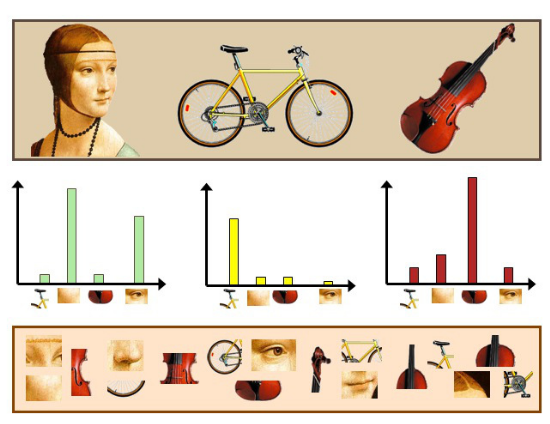
\includegraphics[width=.9\linewidth]{./bagofwords.png} 

\begin{itemize}
\item SIFT detections (green, left) are clustered which gives us a smaller vocabulary
\item On the right, two of the resulting clusters are highlighted
\end{itemize}
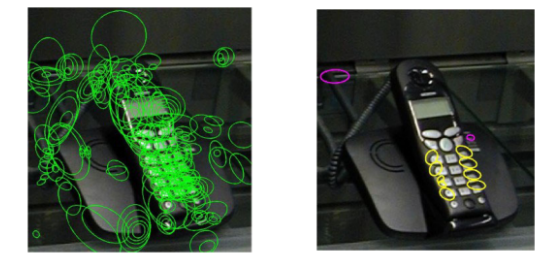
\includegraphics[width=.9\linewidth]{./sift.png}

\subsubsection{Keypoints}
\label{sec-3-5-1}
\begin{itemize}
\item It needs a training set of labelled objects
\item It uses clustering to turn features into visual words
\item It makes no assumption about the spatial relationships between these
\begin{itemize}
\item If a cow is standing on its head, it'll get detected
\item As will a partially separated cow\ldots{}
\end{itemize}
\item Adds a lot of robustness
\item Has a reasonable accuracy of about 80\% on PASCAL VOC
\end{itemize}

\section{Motion Detection}
\label{sec-4}
\begin{itemize}
\item For detecting motion we have two options:
\begin{enumerate}
\item Find the things which aren't moving and ignore them (Background Subtraction)
\item Finding the motion directly (Optical Flow)
\end{enumerate}
\item Once you've found the pixels which represent motion, you need to group them together into 'objects'
\item In relation to the entertainment industry, motion tracking is a huge requirement for when adding post special effects
\begin{itemize}
\item If features cannot be joined up by tracking motion and objects, things look out of sync
\end{itemize}
\end{itemize}

\subsection{Background Subtraction}
\label{sec-4-1}
\begin{itemize}
\item Requires a static camera (all sorts of problems if it isn't)
\item Makes a lot of assumptions
\begin{itemize}
\item The scene is still (mostly)
\item Lighting doesn't change (much)
\item Time series doesn't have a flicker effect anywhere
\end{itemize}
\item Most research in the area deals with violations of these assumptions
\begin{itemize}
\item Always need a static camera though!
\end{itemize}
\end{itemize}
\subsubsection{Work arounds}
\label{sec-4-1-1}
\begin{itemize}
\item A threshold variable is used to ignore small changes in frame-to-frame
\item Lighting is a pain
\item Therefore an adaption is required in all modern forms of Background Subtraction
\item The most simple way to do this is to use an adaptive averaging technique
\begin{itemize}
\item Look back through previous frames, calculate an average and use this as a background
\item This makes new information settle after a time though\ldots{}
\item Two parameters used, threshold $T$ and window $W$ of how many frames to examine for this moving average
\end{itemize}
\end{itemize}
\subsubsection{Flicker}
\label{sec-4-1-2}
\begin{itemize}
\item Often something in the background will cause pixels to vary which we are also not interested in
\begin{itemize}
\item Leaves blowing
\item Camera shakes
\item TV Screens
\item Shadows from outside of the scene
\end{itemize}
\item With flicker, tracking at which point an object appears can be a lot harder
\end{itemize}

\subsubsection{More work arounds}
\label{sec-4-1-3}
\begin{itemize}
\item In situations with flicker and other factors, more complex modelling can be used
\item These generally:
\begin{itemize}
\item Treat each pixel as a time-series
\item Noise processes are modelled explicitly
\item A post-processing step might be used to get rid of small detections
\begin{itemize}
\item Median filters for example
\end{itemize}
\end{itemize}
\end{itemize}

\subsubsection{Additional complications}
\label{sec-4-1-4}
\begin{itemize}
\item It's actually 3D
\begin{itemize}
\item Up until now we consider RGB separately
\begin{itemize}
\item This is a gross oversimplification
\item They quite often vary together
\item It's better to think of each pixel as a point in RGB space
\end{itemize}
\end{itemize}
\item Some objects or noise will vary more than other objects or noise
\begin{itemize}
\item Having a simple threshold means you cannot take this into account
\item Actually, noise is often Gaussian
\item So modelling each pixel as a Gaussian helps
\end{itemize}
\end{itemize}

\paragraph{What does modelling as a Gaussian mean?}
\label{sec-4-1-4-1}
\begin{itemize}
\item We give a standard deviation into the equation, this means our threshold can adjust based on the width of the Gaussian
\item So pixels with a lot of noise have a higher threshold
\end{itemize}

\subsection{Optical Flow}
\label{sec-4-2}

\section{Stereo and Multi-View}
\label{sec-5}
\begin{itemize}
\item Stereo being 2 cameras calibrated
\item Multi-view being $N$ cameras
\begin{itemize}
\item Generally used to build a 3D model of a space
\end{itemize}
\end{itemize}

\section{3D Capture Setups}
\label{sec-6}
\subsection{Vicon make 3D capture}
\label{sec-6-1}
\begin{itemize}
\item One such device is the 'cara' which is a lightweight headset
\item Uses reflective dots on the users face (marker based vision)
\item Uses 3 Cameras (Multiview)
\item Captures facial expressions in real-time
\item Can help build animated models
\end{itemize}
\subsection{Light stage}
\label{sec-6-2}
\begin{itemize}
\item Is a 3D capture system for getting a \emph{detailed} 3D capture model of someones face
\item Used a lot in AAA movies
\item Uses a dome, which has lights and cameras surrounding it
\item Allows you to capture a face under all possible lighting conditions as it cycles through conditions
\item Allows for post production changing of lighting, conditions colours etc all in 3D
\end{itemize}
\section{Background Subtraction/Motion Segmentation}
\label{sec-7}
\begin{itemize}
\item Background subtraction generally relies on a green-screen or a chroma key in order to make things easier
\begin{itemize}
\item This generally means that even if a camera moves, that background subtraction is still possible
\item Being able to do this without a known static background is the "next" step for video production
\end{itemize}
\end{itemize}

\section{VR/AR}
\label{sec-8}
\begin{itemize}
\item Virtual/Augmented Reality is fundamentally dependant on Computer Vision
\end{itemize}
\subsection{Motion tracking}
\label{sec-8-1}
\begin{itemize}
\item For example we require motion tracking for where the user is
\item Where the objects are
\item Where the user is looking (head tracking)
\item Without these, or if done badly or out of sync
\end{itemize}
\subsubsection{Motion sickness}
\label{sec-8-1-1}
\begin{itemize}
\item B. Allen et al. Visual 3D acuity predicts discomfort in 3D stereoscopic environments. Entertainment Computing.
\item Reports that 78\% of women and 33\% of men felt ill from using the HTC Vive
\item Can stem from a discontinuity between motion being made and one being shown
\end{itemize}
% Emacs 25.2.2 (Org mode 8.2.10)
\end{document}